\subsection{角的和、差与画法}\label{subsec:czjh1-1-7}

和线段一样,对于任意两个角也可以进行加、减,得出新的角。
一个角的度数是另两个角度数的和(或差), 这个角就是另两个的和(或差)。

下面我们来学习利用量角器画一个角及画两个角的和、差的方法。

\liti 已知 $\angle AOB$, 用量角器画一个角等于 $\angle AOB$。

\huafa 1. 用量角器量得 $\angle AOB = 41^\circ$(图 \ref{fig:czjh1-1-29})。

\begin{figure}[htbp]
    \centering
    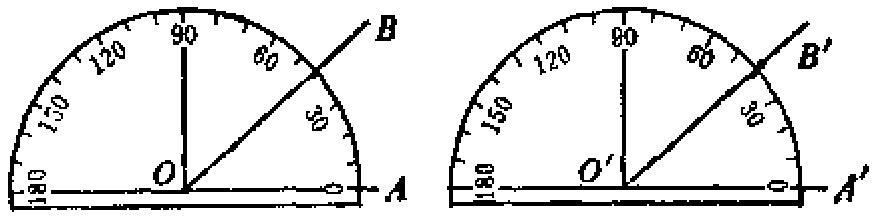
\includegraphics[width=8cm]{../pic/czjh1-ch1-29.png}
    \caption{}\label{fig:czjh1-1-29}
\end{figure}

2. 画射线 $O'A'$。

3. 用量角器画 $\angle A'O'B' = 41^\circ$。

$\angle A'O'B'$ 就是所求的角。

用量角器画 $\angle A'O'B' = 41^\circ$ 是这样画的:
先将量角器的中心对准点 $O'$, 将标有 $0$ 的线对准 $O'A'$,
然后在量角器上找出 $41^\circ$ 线,靠它的外端画一个点 $B'$,画射线 $O'B'$。
$\angle A'O'B'$ 就等于 $41^\circ$。

\begin{figure}[htbp]
    \centering
    \begin{minipage}[b]{7cm}
        \centering
        \begin{tikzpicture}
	\pgfmathsetmacro{\r}{2.5}
	\pgfmathsetmacro{\R}{3.5}
	\pgfmathsetmacro{\a}{30}
	\pgfmathsetmacro{\b}{45}

	\begin{scope} [xshift=-1cm]
		\tkzDefPoints{0/0/B, \r/0/A}
		\tkzDefPoint(\a:\r){C}
		\tkzDrawSegments(B,A  B,C)
		\tkzMarkAngle[size=0.5](A,B,C)
		\tkzLabelAngle[pos=0.8](A,B,C){$1$}
	\end{scope}

	\begin{scope} [xshift=2cm]
		\tkzDefPoints{0/0/B, \r/0/A}
		\tkzDefPoint(\b:\r){C}
		\tkzDrawSegments(B,A  B,C)
		\tkzMarkAngle[arc=ll, size=0.5](A,B,C)
		\tkzLabelAngle[pos=0.8](A,B,C){$2$}
	\end{scope}

	\begin{scope} [yshift=-4cm]
		\tkzDefPoints{0/0/B, \R/0/A}
		\tkzDefPoint(\a:\R){C}
		\tkzDefPoint(\a+\b:\R){D}
		\tkzDrawSegments(B,A  B,C B,D)
		\tkzMarkAngle[size=0.5](A,B,C)
		\tkzMarkAngle[arc=ll, size=0.8](C,B,D)
		\tkzLabelPoints[below](B, A)
		\tkzLabelPoints[right](C, D)
	\end{scope}
\end{tikzpicture}


        \caption{}\label{fig:czjh1-1-30}
    \end{minipage}
    \qquad
    \begin{minipage}[b]{7cm}
        \centering
        
\begin{tikzpicture}
	\pgfmathsetmacro{\r}{2.5}
	\pgfmathsetmacro{\R}{3.5}
	\pgfmathsetmacro{\a}{70}
	\pgfmathsetmacro{\b}{30}

	\begin{scope} [xshift=-1cm]
		\tkzDefPoints{0/0/B, \r/0/A}
		\tkzDefPoint(\a:\r){C}
		\tkzDrawSegments(B,A  B,C)
		\tkzMarkAngle[size=0.5](A,B,C)
		\tkzLabelAngle[pos=0.8](A,B,C){$1$}
	\end{scope}

	\begin{scope} [xshift=2cm]
		\tkzDefPoints{0/0/B, \r/0/A}
		\tkzDefPoint(\b:\r){C}
		\tkzDrawSegments(B,A  B,C)
		\tkzMarkAngle[arc=ll, size=0.5](A,B,C)
		\tkzLabelAngle[pos=0.8](A,B,C){$2$}
	\end{scope}

	\begin{scope} [yshift=-4cm]
		\tkzDefPoints{0/0/B, \R/0/A}
		\tkzDefPoint(\a:\R){C}
		\tkzDefPoint(\b:\R){D}
		\tkzDrawSegments(B,A  B,C B,D)
		\tkzMarkAngle[size=0.5](A,B,C)
		\tkzMarkAngle[arc=ll, size=0.8](A,B,D)
		\tkzLabelPoints[below](B, A)
		\tkzLabelPoints[right](C, D)
	\end{scope}
\end{tikzpicture}


        \caption{}\label{fig:czjh1-1-31}
    \end{minipage}
\end{figure}

\liti 已知 $\angle 1$、$\angle 2$。 用量角器画一个角,使它等于 $\angle 1 + \angle 2$。

\huafa  1. 用量角器画 $\angle ABC = \angle 1$(图 \ref{fig:czjh1-1-30} )。

2. 以点 $B$ 为顶点, 射线 $BC$ 为一边, 画 $\angle CBD = \angle 2$, 并且使射线 $BD$ 在 $\angle ABC$ 的外部。

$\angle ABD$ 就是所求的角。



\liti 已知 $\angle 1$、$\angle 2$, 且 $\angle 1 > \angle 2$。 用量角器画一个角,使它等于 $\angle 1 - \angle 2$。

\huafa 1. 用量角器画 $\angle ABC = \angle 1$ (图 \ref{fig:czjh1-1-31} )。

2. 以点 $B$ 为顶点, 射线 $BA$ 为一边画 $\angle ABD = \angle 2$,并且使射线 $BD$ 在 $\angle ABC$ 的内部。

$\angle CBD$ 就是所求的角。


画两角的和或差,也可以先计算出两角的度数的和或差后,再利用量角器画这个角。

\begin{enhancedline}
如果 $\angle \alpha$ 是 $n$ 个 $\angle \beta$ 的和,
那么我们就说 $\angle \alpha$ 是 $\angle \beta$ 的 $n$ 倍或 $\angle \beta$ 是 $\angle \alpha$ 的 $n$ 分之一。
记作 $\angle \alpha = n \angle \beta$ 或 $\angle \beta = \exdfrac{1}{n} \angle \alpha$。

从一个角的顶点引出的一条射线,把这个角分成两个相等的角,这条射线叫做这个\zhongdian{角的平分线}。
如图 \ref{fig:czjh1-1-32} , 射线 $OK$ 把 $\angle GOH$ 分成两个相等的角,它是 $\angle GOH$ 的平分线。
记作 $\angle GOK = \angle KOH$ 或 $\angle GOK = \exdfrac{1}{2} \angle GOH$ 或 $\angle GOH = 2 \angle GOK ( = 2 \angle KOH)$。

\begin{figure}[htbp]
    \centering
    \begin{minipage}[b]{7cm}
        \centering
        \begin{tikzpicture}
	\pgfmathsetmacro{\R}{2.5}
	\tkzDefPoints{0/0/O, \R/0/G}
	\tkzDefPoint(30:\R){K}
	\tkzDefPoint(60:\R){H}
	\tkzDrawSegments(O,G  O,K  O,H)
	\tkzMarkAngle[size=0.5](G,O,H)
	\tkzLabelPoints[left](O)
	\tkzLabelPoints[below](G)
	\tkzLabelPoints[right](H, K)
\end{tikzpicture}


        \caption{}\label{fig:czjh1-1-32}
    \end{minipage}
    \qquad
    \begin{minipage}[b]{7cm}
        \centering
        \begin{tikzpicture}
	\pgfmathsetmacro{\R}{2.5}
	\tkzDefPoints{0/0/B, \R/0/A}
	\tkzDefPoint(21:\R){D}
	\tkzDefPoint(42:\R){C}
	\tkzDrawSegments(B,A  B,D  B,C)
	\tkzLabelPoints[left](B)
	\tkzLabelPoints[right](A, C, D)
\end{tikzpicture}


        \caption{}\label{fig:czjh1-1-33}
    \end{minipage}
\end{figure}

\liti 已知 $\angle ABC$, 画它的角平分线。

\huafa 1. 量得 $\angle ABC = 42^\circ$(图 \ref{fig:czjh1-1-33} ),求得 $\exdfrac{1}{2} \angle ABC = 21^\circ$。

2. 以点 $B$ 为顶点, $AB$ 为一边, 在 $\angle ABC$ 的内部画 $\angle ABD = 21^\circ$。

射线 $BD$ 就是所求的角平分线。
\end{enhancedline}


\begin{lianxi}

\xiaoti{已知 $\angle \alpha < 90^\circ$, 画一个角, 使它等于 $2 \angle \alpha$。}

\xiaoti{用一块三角板画一个 $90^\circ$ 的角,再画它的角平分线。}

\xiaoti{用量角器和直尺画一个角等于 $84^\circ$, 再这个角三等分。}

\xiaoti{一副三角板中, 一块三角板的三个角是 $30^\circ$、$60^\circ$、$90^\circ$,
    另一块三角板的三个角是 $45^\circ$、$45^\circ$、$90^\circ$。
    利用三角板画等于下列度数的角; $30^\circ$、$75^\circ$、 $105^\circ$、 $15^\circ$。
}

\end{lianxi}


